\chapter{Introduction}
%\section{Introduction}
Starting in the 19th century, the physical worldview was based on following theories:
\begin{itemize}
    \item Mechanics (Newton)
    \item Electrodynamics (...., Coulomb, Ampere, Faraday, Maxwell)
    \item Thermodynamics (...., Boltzmann)
\end{itemize}
The existence of atoms/molecules has just been accepted by physicists, the dispute among the chemists was still open. The Avogadro/Loschmidt's number of molecules per mole was found to be N $\sim {10}^{22}-{10}^{24}$
(today N = $6.02\cdot10^{23}$) estimated and for the radius of the H-Atoms/$H_{2}O$ molecules
The estimates ranged from $1 - 2\cdot10^{-8} $cm, ie.
1-2 $\dot{A}$. In the period from about 1900 to 1930 a number of experiments, which were in clear contradiction to the classical worldview. These
experiments seemed to show (and indeed did) that
\begin{center}
(Light-) waves $\to$  are Particles,\\
Particles $\to$  are Waves,
\end{center}
and that quantization of physical quantities such as energy or angular momentum occurs. The explanation of all these experiments by the (new) Quantum mechanics based on the work of Heisenberg, 1925 ($\gets$Bohr, Born, Jordan, Pauli) and his rival Schrodinger, 1926 ($\gets$de Broglie, Einstein) is probably the greatest triumph of physics in the last century. Heisenberg's (abstract) matrix formalism and Schrodinger's (illustrative) wave mechanics turned out to be equivalent (Schrodinger
1926) and formed together with the Copenhagen interpretation
(Heisenberg'sche Unsch arferelation, Bohr, Born, ...) the foundations of
Quantum mechanics as we know it today. In the following we discuss
some key experiments that inspired the development of quantum mechanics
to have.

\section{1900 Planck's law of radiation}
Consider a cavity ($V = L^3$) of temperature T. The classical Rayleigh-Jeans law for the spectral energy density $u(w)$ [Energy/Volume Hz] follows from the counting of the free electromagnetic modes and the fact that classically every fashion carries the energy $k_BT$. One simple argument for counting the modes in volume V is provided by the Application of periodic boundary conditions for the vector potential, $\vec{A}=\sum_{\vec{k}} \vec{A}_{\vec{k}} \exp (i \vec{k} \cdot \vec{r}) \text { with } \vec{k} \cdot \vec{A}_{\vec{k}}=0$ ($\vec{A}$ is transversal) and $\vec{A}_{-\vec{k}}=\vec{A}_{\vec{k}}^{*}$ ($\vec{A}$ is real). Allowed $\vec{k}-$ values are $\vec{k}=(2 \pi / L) \vec{n}$ with $n_i$ all and we get the Number of dN modes in the interval $[k, k+ dk]$ (factor 2 for two transversal Directions, factor 2 for $\vec{A}_{\vec{k}}$ complex, factor 1/2 for $\vec{A}$ real)
\begin{equation} \label{0.1}
d N=2 \cdot 2 \cdot \frac{1}{2} \cdot \frac{4 \pi k^{2}}{(2 \pi / L)^{3}} d k
\end{equation}
If you want to find the physically correct modes you have to do more work. We take an ideal metallic cavity at dimension $L^2d$ ($d = L $ at the end) and TE (transversal electrical) and TM (transversal
magnetic) modes (see electrodynamics lecture or J. D. Jackson,
Classical Electrodynamics),
\begin{equation}
\begin{array}{c}{\mathrm{TE}: H_{z} \propto \cos (m \pi x / L) \cos (n \pi y / L) \sin (p \pi z / d)} \\ {m, n \mbox  { for all, not both }=0, p \neq 0 \mbox{ for all}}\end{array}
\end{equation}
\begin{equation}
\begin{array}{c}{\mathrm{TM}: E_{z} \propto \sin (m \pi x / L) \sin (n \pi y / L) \cos (p \pi z / d)} \\ {m, n \neq 0 \mbox{ for all}, p \mbox  { for all }}\end{array}
\end{equation}
%公式0.2,0.3
The components $\vec{H}_{\bot}$ and $\vec{E}_{\bot}$ follow from $\nabla_{\bot}H_z$ and $\nabla_{\bot}E_z$. Then counting the allowed values for $m,n,p$ (with $ d = L$) then yields $dN = (1/8)\cdot 2 \cdot 4\pi k^2 / (\pi/L)^3 dk$, in agreement with (Formula 0.1) (factor 1/8 for one octant, factor 2 for TE and TM modes).
%图1
\begin{figure}[ht]
    \centering
    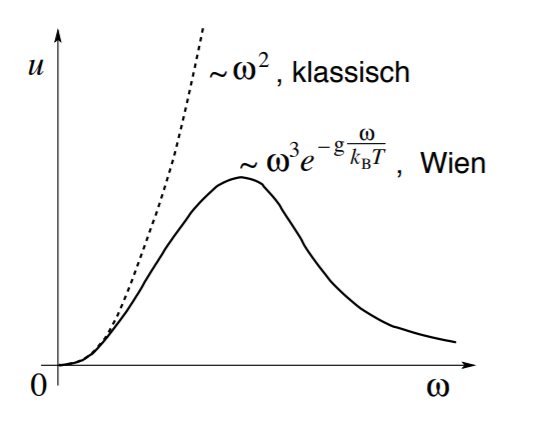
\includegraphics[scale=1]{1.PNG}
    \captionsetup{font={Large}}
    \caption{Spectral energy density $u(w)$. The classically unlimited energy density (dotted) saturates in reality (extended) and falls exponentially to zero at high energies (Wien and Planck's law of radiation).}
    \label{fig:1}
\end{figure}
In thermodynamic equilibrium at the temperature T, each mode carries an energy $k_BT$ ($k_B = 0.8617 10^{-4} eV/K$) designates the Boltzmann
Constant) and with the dispersion $w = ck (c = 2.998 10^8 m/s$, the speed of light). For light, the spectral energy density results:
\\\begin{equation}
u(\omega) d \omega=\frac{k_{\mathrm{B}} T}{\pi^{2} c^{3}} \omega^{2} d \omega
\end{equation}

%公式0.4
This results in the ultraviolet catastrophe:
\begin{equation}
\int_{0}^{\infty} d \omega u(\omega)=\infty
\end{equation}
%公式0.5
However, experiments and empirical analyzes show (Vienna) that
\begin{equation}
u(\omega) \sim\left\{\begin{array}{ll}{\omega^{2},} & {\omega \rightarrow 0} \\ {\omega^{3} e^{-g \omega / k_{\mathrm{B}} T},} & {\omega \rightarrow \infty}\end{array}\right.
\end{equation}
%公式0.6
as shown in Figure 1. The constant $g$ has the dimension energy times, which gives an effect; you determine them via comparison with experiments. Find Planck's Law of Radiation based on the hypothesis that matter only radiation in quanta of $\hbar w$ releases;
Under this assumption we find the new expression for the spectral energy density
\begin{equation}
u(\omega)=\frac{\hbar}{\pi^{2} c^{3}} \frac{\omega^{3}}{e^{\hbar \omega / k_{\mathrm{B}} T}-1}
\end{equation}
with
\begin{equation}
 \hbar=6.58210^{-16} e \mathrm{Vs}=1.05510^{-34} \mathrm{Js}
\end{equation}
%公式0.7,0.8
The comparison with the experiment gives a first indication of the quantization of the radiation field.(Modern formulation: the mode with$w = ck$ is using a number of quanta $\langle n\rangle$)


%PAGE 4
\section{1905 Photoelectric effect(Einstein)}
Becomes a (metallic) upper ache by light ((circle) frequency $w$, visible or UV) (Hertz, Lenard) you find an upper limit
\begin{equation}
E_{\mathrm{kin}}=\frac{m v^{2}}{2}=\hbar \omega-W
\end{equation}
%公式0.10
for the kinetic energy of electrons ($\gets$ J.J. Thompson, 1897, Elektronen as constituents of the atoms: J.J. Thompson $\sim$1899). $W$ is the work function, with a value in the size order $eV$. Classic would expect another result: the intensity of the radiation is increased by their energy flux density $\vec{S} = (c/4\pi)\vec{E}\times \vec{H}$ characterized. The continuous absorption of this radiation can be expected that $i$) no upper bound
for the kinetic energy $E_{kin}$ exists, $ii$) no lower bound for $w$ occurs, and $ iii$) a delayed emission at low intensity (proportional
to the energy density $(E^2 + H^2) /8\pi$) occurs. Instead, you find as shown in Figure 2, the photocurrent starts immediately when $\hbar w > W$
(lower bound for $w$) and $E_{kin}$ is limited. It can be concluded that light consists of photons (energy quanta of energy $\hbar w$). Spater de Broglie and Compton showed that the light waves correspond to particles with\\
\begin{equation}
\begin{array}{l}{\mbox { Impulse: } \vec{p}=\hbar \vec{k}, \quad \omega=c k} \\ {\mbox  { Energy : } E=\hbar \omega} \\ {\mbox  { Foursome pulse: }\left(\begin{array}{c}{E / c} \\ {\vec{p}}\end{array}\right)=\hbar\left(\begin{array}{c}{k} \\ {\vec{k}}\end{array}\right)}\end{array}
\end{equation}
%公式0.11
occupied by the given
\\
\begin{equation}
    \langle n(\omega)\rangle \sim \frac{\sum_{n} n e^{-\beta n \hbar \omega}}{\sum_{n} e^{-\beta n \hbar \omega}}=\left.\left(1-e^{-y}\right)\left(-\partial_{y}\right)\left(1-e^{-y}\right)^{-1}\right|_{y=\beta \hbar \omega}=\frac{1}{e^{\hbar \omega / k_{\mathrm{B}} T}-1}
\end{equation}\\
%公式0.9 
with $\beta = 1/k_BT$. Each mode then carries an energy $\hbar w\langle n(w)\rangle$ to the energy density of the
radiation field at. For small energies $\hbar w <k_BT$ can be the exponential function in $\langle n(w)\rangle$ develop and you will continue to find the contribution $\hbar w\langle n(w)\rangle \approx k_BT$, during modes with $\hbar w > k_BT$ contributes little exponentially. Task: Compare $\langle E\rangle_{classical}$, and $\langle E\rangle_{qm}$.

%Page 5
%图2
\begin{figure}[ht]
    \centering
    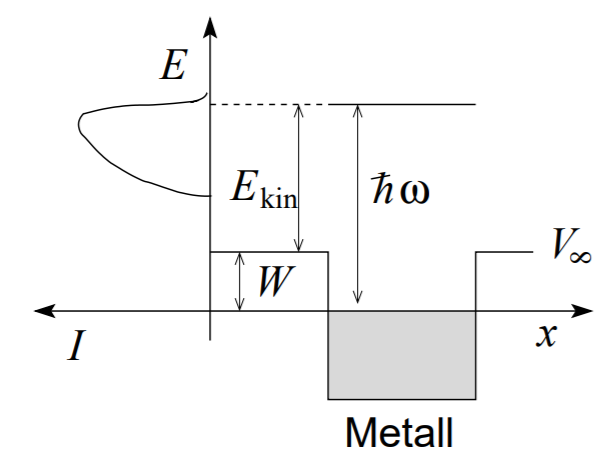
\includegraphics[scale=1]{2.PNG}
    \captionsetup{font={Large}}
    \caption{Photons of energy $\hbar w$ strike electrons from a metal. The intensity (left) of the emitted electrons is limited by the band edge (bottom) and by the Fermi energy of the metallic electrons (top).}
    \label{fig:2}
\end{figure}
\section{1907 Special Warmth of the Festival (Einstein)}
The quantization of the excitations (phonons) in the solid state is in the treatment of the cavity radiation/Planck's law of radiation similar;Differences are in the spectrum (dispersion) and in the finite number of modes (finite number of atoms, finite grid instead of continuous vacuum). We will not go back to it.

\section{1913 Bohr quantization of the atom}
Starting point is the Rutherford atom with small, positively charged core (extension $\sim10^{-13} - 10^{-12}$ cm) orbited by (negatively charged) electrons (J.J. Thompson, 1899). The formula $v=R(1/n^2 - 1/m^2), R = \text{Rydberg Constant}, m, n$ for all, for the Balmer series describes the frequencies the observed spectral lines. Classically, the electron moves in a circular path and is thus accelerated.\\
Due to this orbital motion, the atom emits energy off and the electron should (with emission of continuous radiation) to the core. Bohr postulates that atom exists only in stationary or quantum states of well-defined energy. The sharp spectral lines are then the consequence of transitions between these states.
\\
\begin{equation}
\hbar \omega=\left|E_{f}-E_{i}\right|, \quad \begin{array}{ll}{\text { Absorption : }} & {E_{i}<E_{f}} \\ {\text { Emission: }} & {E_{i}>E_{f}}\end{array}
\end{equation}\\
%公式0.12
where $i,f$ for the $i$ initial, $f$ final state. The ground state $E_0 =min (E_i)$ is stable. For the hydrogen atom applies \\
\begin{equation}
E_{n}=-\hbar \frac{2 \pi R}{n^{2}}, \quad n=1,2,3, \ldots
\end{equation}\\
%公式0.13
from which the Balmer formula results.

\section{1914 Franck-Hertz experiment}
The experiment, see Figure  3, underlines the existence of discrete energy levels in atoms. The structure (peaks) in the observed current
%图3
\begin{figure}[ht]
    \centering
    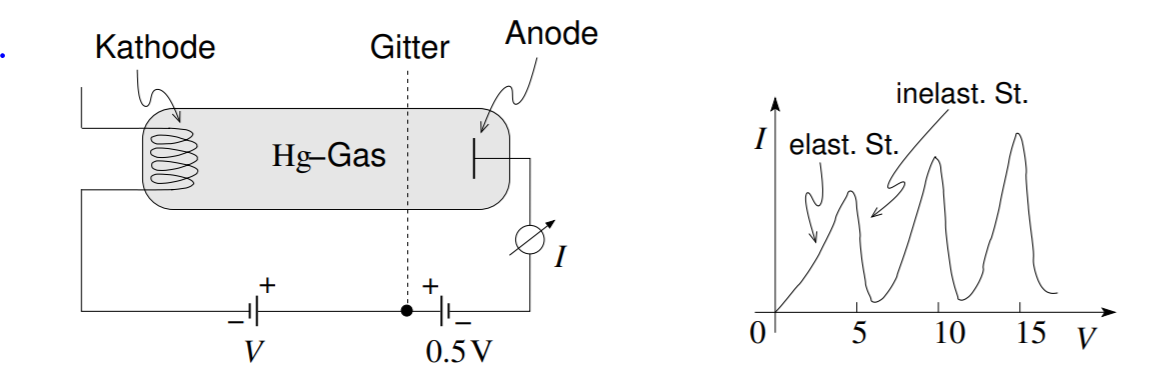
\includegraphics[scale=1]{3.PNG}
    \captionsetup{font={Large}}
    \caption{Electrons accelerated by an electric potential hit Hg atoms. Inelastic shocks transfer the atoms into high-energy excited states, which decay under the emission of electromagnetic radiation.}
    \label{fig:3}
\end{figure}
versus voltage characteristic is interpreted as follows: electrons take in the potential $V$ kinetic energy, which they release to the same through inelastic collision with the Hg atoms. The atoms are from the ground state with energy $E_0$ in an excited state with energy $E_n, E_n - E_0 \approx 5 eV$ lifted. The stopped electrons reach the anode no more and there are peaks in $I (V)$; the atoms are falling emission of radiation back to the ground state.

\section{1922 Stern-Gerlach experiment}
Paramagnetic atoms with magnetic moment $\vec{\mu} = \mu_0 \vec{L}, \vec{L}$ the angular momentum, are exposed to an inhomogeneous magnetic field $\vec{B}$ and their distraction is measured. Classically, the following behavior is expected:
%图4
\begin{figure}[ht]
    \centering
    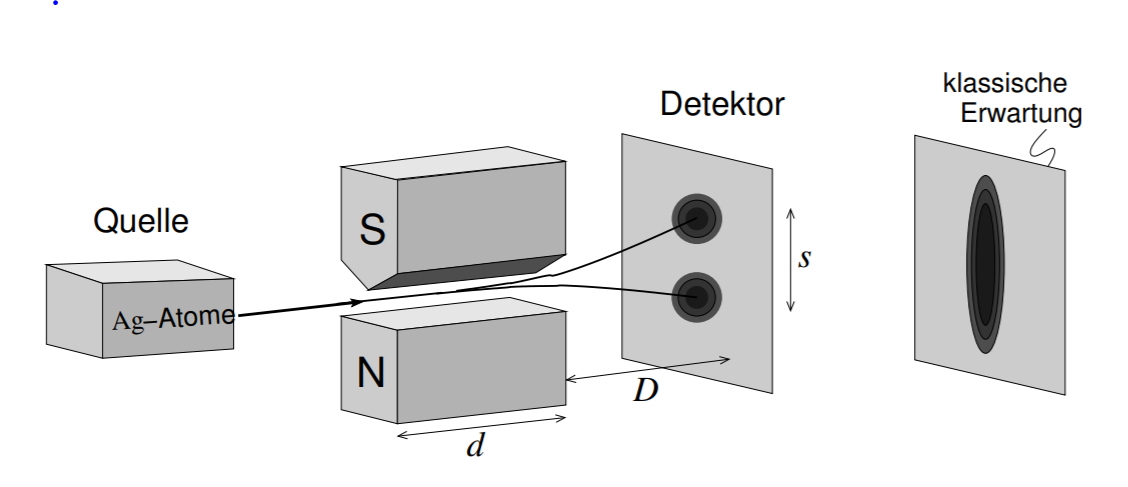
\includegraphics[scale=1]{4.PNG}
    \captionsetup{font={Large}}
    \caption{Paramagnetic atoms with magnetic moment $\vec{\mu}=\mu_0 \vec{L}$= angular momentum and (thermal) energy $E = mv^2/2 \approx k_BT$ are deflected in an inhomogeneous magnetic field. Discrete spots are observed at the detector instead of the traditionally expected continuous distribution.}
    \label{fig:4}
\end{figure}
the energy in the magnetic field $E_{magn}=-\vec{\mu}\cdot \vec{B}$ yields the force $\vec{F}=\bigtriangledown(\vec{\mu}\cdot\vec{B})$. Here is $F_z=\mu_z\partial_zB$, for example, and that's the reason for the distraction on the screen
$s=(\mu_z\partial_zBd/2k_BT)(d/2+D)$. Since (classical) the angular momentum $L_z$ along $z$ is continuously distributed, it would be a continuous distribution of
atoms along $z$ direction, see Figure  4, in contradiction to the factual observed quantized results with discrete patches. Consequently, the angular momentum of atoms quantized.

\section{1923/25 Compton Effect (Compton and Debye)}
In this experiment, light rays are scattered by electrons, the geometry sketched in Figure  5.
Classically, the following results are expected: a continuous pulse transfer from the radiation field to the electron (the radiation pressure causes the momentum $p_e$ of the electron to grow continuously with the irradiation time); all electrons are accelerated equally; the absorption and re-emission of radiation by the electron takes place in (momentary)
Resting system of the electron at the same wavelength. The Doppler effect then produces a (angle-dependent) wavelength shift $\triangle \lambda $ ($\lambda$ is the wavelength of the incident beam),\\
\begin{equation}
\Delta \lambda=2 \lambda \frac{c p_{\mathrm{e}}}{E_{\mathrm{e}}-c p_{\mathrm{e}}} \sin ^{2} \frac{\theta}{2}, \quad \vartheta=0, \quad E_{\mathrm{e}}^{2}=m_{\mathrm{e}}^{2} c^{4}+p_{\mathrm{e}}^{2} c^{2}
\end{equation}\\
%公式0.14
In fact, however, you find the shift
\\
\begin{equation}
\Delta \lambda=4 \pi \frac{\hbar}{m_{\mathrm{e}} c} \sin ^{2} \frac{\theta}{2}
\end{equation}\\
%公式0.15
with the new parameter $\hbar/m_ec= 3.86\times10^{-11}$ cm, the Compton Wavelength of the electron. Also, one notices that not all electrons accelerated simultaneously and evenly: only those electrons which absorb a photon, have a pulse $p_e \neq 0$ and also
this pulse varies discretely. These results indicate that the light is in the scattering process corresponds to a particle, although the light clearly has wave character, comparing to other experiments with light, e.g. the Double-slit experiment or the action on crystals (von Laue, 1912). The experiment thus points to a particle/wave duality for the radiation.
%图5
\begin{figure}[ht]
    \centering
    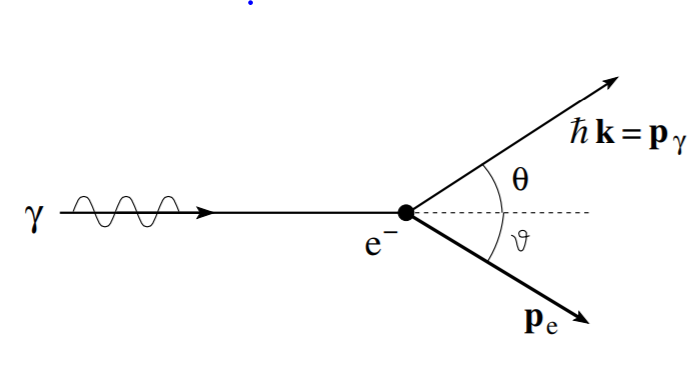
\includegraphics[scale=1]{5.PNG}
    \captionsetup{font={Large}}
    \caption{X-rays (photons) strike a resting electron $e^-$ and are scattered.}
    \label{fig:5}
\end{figure}
The assumption that the scattering process as particles-particles (i.e., photon-electron) scattering with momentum and energy conservation (4-invariant)
can lead to the correct result (0.15): the four-momentum remains in the scattering process,
\\
\begin{equation}
\begin{array}{l}{\text { initial: }\left(\begin{array}{c}{\hbar k} \\ {\hbar \vec{k}}\end{array}\right)+\left(\begin{array}{c}{m_{\mathrm{e}} c} \\ {0}\end{array}\right), 
\quad \text { final: }\left(\begin{array}{c}{\hbar k^{\prime}} \\ {\hbar \overrightarrow{k^{\prime}}}\end{array}\right)+\left(\begin{array}{c}{\sqrt{p_{\mathrm{e}}^{2}+m_{\mathrm{e}}^{2} c^{2}}} \\ {\hbar \overrightarrow{k^{\prime}}}\end{array}\right)%+\left(\begin{array}{c}{\sqrt{p_{\mathrm{e}}^{2}+m_{\mathrm{e}}^{2} c^{2}}} \\ {\overrightarrow{p_{\mathrm{e}}}}\end{array}\right)
} 
\\ {\left(\begin{array}{c}{\hbar\left(k-k^{\prime}\right)+m_{\mathrm{e}} c} \\ {\hbar\left(\vec{k}-\vec{k}^{\prime}\right)}\end{array}\right)=\left(\begin{array}{c}{\sqrt{p_{\mathrm{e}}^{2}+m_{\mathrm{e}}^{2} c^{2}}} \\ {\vec{p}_{\mathrm{e}}}\end{array}\right)}\end{array}
\end{equation}
%公式0.16,
and the four-squares product $a^{\mu}a_{mu}=a^0a_0-\vec{a}\cdot\vec{a}$ are
\begin{equation}
k-k^{\prime}=\frac{\hbar}{m_{\mathrm{e}} c} k k^{\prime}(1-\cos \theta)
\end{equation}
%公式17
The result (0.15) then follows with the assumption $k = 2\pi/\lambda$. The experiment attests to the light a particle character
\\
\begin{equation}
\begin{aligned} E &=\hbar \omega \\ \vec{p}_{\gamma} &=\hbar \vec{k}=\vec{p}, \quad \quad P^{\mu}=\left(\begin{array}{c}{E / c} \\ {\vec{p}}\end{array}\right)=\hbar\left(\begin{array}{c}{k} \\ {\vec{k}}\end{array}\right) \\ \vec{p} / p &=\text { propagation } \\ \omega &=c k \end{aligned}
\end{equation}
%公式0.18

\section{1923 de Broglie hypothesis}
Matter and radiation behave the same (universal) and show both wave and particle character,
\begin{equation}
\begin{array}{l}{\text { Wave } \longrightarrow \text { Particle } \stackrel{\text { DeB }}{\rightarrow} \text { Wave }} \\ {\qquad(h=2 \pi \hbar)}\end{array}
\end{equation}\\
%公式0.19
That a wave behaves like a particle follows from the photoelectric effect and the Compton scatter. De Broglie rearranges the particle with momentum$ p$
, a wave with wavelength $\lambda=h/p$ too.

\section{1923 Bohr's correspondence principle}
Classical theory is macroscopic and special in all (for example in the description of electrons in static electromagnetic field) also microscopically correct. On the other hand, the classical theory fails when quantum disciplines become relevant. The quantum theory must reproduce the results of classical theory in the limit of large quantum numbers(corresponding to small quantum discontinuity). Consequently, there must be a formal analogy between quantum theory and classical theory. These arguments form the basis for the correspondence principle. \\\\
As an example, consider the Bohr atom with the energies $E_n=hR/n^2$, see Figure  6. R is an unknown proportionality constant. The classical analogue is the Kepler problem with the gravitational potential
replaced by the electrical potential $-e^2/r$. The Kepler law for the rotational frequency $v(E) = 1/T$, $T$ the orbital period, $E$, the energy of the
%PAGE 10
classic elliptical orbit, is (transferred to the electronic potential)
\begin{equation}
\nu=\frac{1}{\pi e^{2}}\left(\frac{2|E|^{3}}{m}\right)^{1 / 2}
\end{equation}
%公式0.20
On the other hand, a quantum mechanical view of the spectrum results at high energies the (energy-dependent) fundamental frequency
\begin{equation}
\nu\left(E_{n}\right)=\frac{E_{n+1}-E_{n}}{h} \approx \frac{1}{h} \frac{d E_{n}}{d n}(\Delta n=1)=\frac{2 R}{n^{3}}=2\left(\frac{\left|E_{n}\right|^{3}}{R h^{3}}\right)^{1 / 2}
\end{equation}
%公式0.21
where we have used the dependency $E_n = hR/n^2$. The relevant frequencies in the radiation at high energies are then given by $[E_{n+\triangle n}-E_n=v_{\triangle n}(E)=\triangle n v(E)]$, provided that $\triangle n/n \ll 1$ satisfied.
%图6
\begin{figure}[ht]
    \begin{minipage}{0.5\textwidth}
        \centering
        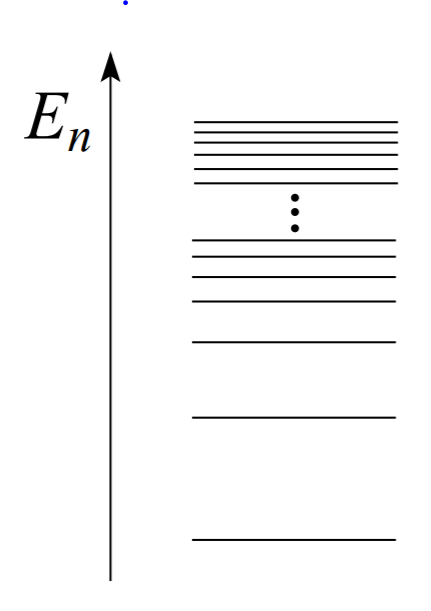
\includegraphics[scale=1]{6.PNG}
    \end{minipage}
    \begin{minipage}{0.5\textwidth}
        \captionsetup{font={Large}}
        \caption{Discrete spectrum in Bohr's atomic model. The correspondence principle can be applied to high excitation energies $E_n$ with $n\gg 1$, where the spectrum is quasi-continuous.}
    \end{minipage}
    \label{fig:6}
\end{figure}
From the correspondence between the Kepler problem (0.20) and the quantum mechanical problem (0.21) we get an expression for the constant $R$\\
\begin{equation}
\begin{aligned} \nu_{\mathrm{Kep}} &=\frac{1}{\pi e^{2}}\left(\frac{2|E|^{3}}{m}\right)^{1 / 2}=2\left(\frac{|E|^{3}}{R h^{3}}\right)^{1 / 2}=\nu_{q} \\ & \rightarrow R=\frac{2 \pi^{2} m e^{4}}{h^{3}}, \quad E_{n}=-\frac{m e^{4}}{2 \hbar^{2}} \frac{1}{n^{2}}=-\frac{13.6 \mathrm{eV}}{n^{2}} \end{aligned}
\end{equation}\\
%公式0.22
We briefly check the dimensional correctness of the result: the ground state is characterized by the potential and kinetic energies $E_{pot}\approx -e^2/r$ and $E_{kin} = p^2/2m \approx \hbar^2\pi^2/2mr^2$, where we
%PAGE 11
have used the blurring relation in the form $p\cdot r\sim\pi\hbar$. Put
we $E_{kin}\approx -E_{pot}$ (virial theorem), we get $r \approx \hbar^2\pi^2/2me^2$ and
$E \approx -2me^4/\pi^2\hbar^2$, which is a factor $4/\pi^2\approx 0.4$ .

\section{1925 Matrix Mechanics (Heisenberg)}
See detailed discussion later.
\section{1926 Wave mechanics (Schrodinger)}
See detailed discussion later.
\section{1927 Davisson and Germer experiment}
We consider the scattering experiment analogous to the Laue experiment but with particles. The reflection of electrons from a crystal survey yields `von Laue' reflection as sketched in Figure  7. 
%图7
\begin{figure}[ht]
    \centering
    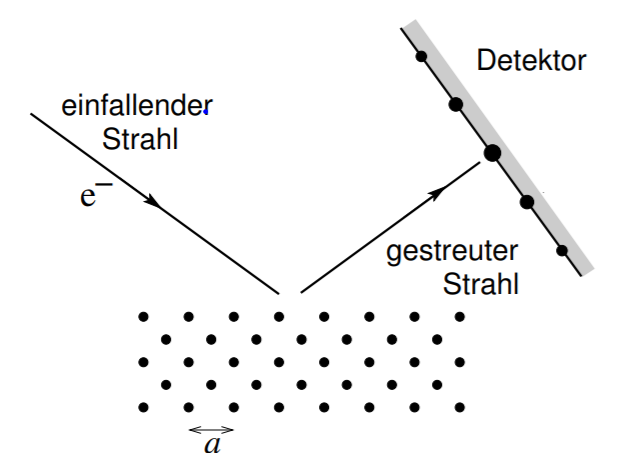
\includegraphics[scale=1]{7.PNG}
    \captionsetup{font={Large}}
    \caption{Scattering of electrons on a crystal surface.}
    \label{fig:7}
\end{figure}
The needed wavelength and energy of the electrons are obtained from the de Broglie Relationship (use that $\hbar\cdot \hbar=6.58\times 10^{-16}eVs \cdot 1.055\times 10^{-34}Js$)
\\\begin{equation}
\lambda=\frac{2 \pi \hbar}{p}=\frac{2 \pi \hbar}{\sqrt{2 m E}}=\frac{12.2 \mathrm{A}}{\sqrt{E[\mathrm{eV}]}}
\end{equation}
\\
%公式0.23
The lattice constant $a \sim5 \overset{\circ}{A} $leads to an energy $E$ of a few $eV$; This is just the typical energy scale of the electrons in the crystal (The electrons in the crystal are compatible with a crystal structure of length scale $a$).\\\\
%PAGE 12
Conversely, the structure of the Laue interference image confirms the validity of the De Broglie relation $\lambda = h/p$ (the interference pattern gives a value of the compatible $\lambda$ with the energy $E$ of the scattered electrons).
\section{1913-1927 Bohr-Sommerfeld Quantization and `old' quantum mechanics}
The correspondence principle and the Bohr quantization lead to a selection criterion for classical orbits permitted in quantum mechanics: select those orbits which satisfy a quantization condition (the criterion works for periodic orbits). This gives us the transition from continuous to quantized results. The desired quantization must have something to do with Planck's quantum effect. Dimensionally, $[h]$ = effect, so the effect of the orbit is to be quantized. Returning to Lagrangian mechanics, a mechanical problem is defined by the coordinate $q$ and the Lagrange function $\mathcal{L}$. The conjugate momentum is given as the derivative $p = \partial \mathcal{L}/\partial q$, and the effect of a trajectory is given by the time integral
\begin{equation}
\mathcal{S}=\oint d t \mathcal{L}=\oint d q p-E \oint d t
\end{equation}
%公式0.24
where we have separated the district. The latter we quantify according to
\begin{equation}
\oint d q p=n h
\end{equation}
%公式0.25
with $n \in N$. In the example the hydrogen atoms become the radial and azimuthal ones track shares quantized,$\oint d r p_{r}=k h$and$\oint d \varphi p_{\varphi}=l h$. We choose
a fixed orbital plane; with $\mathcal{L}=(m / 2)\left[\dot{r}^{2}+(r \dot{\varphi})^{2}\right]+e^{2} / r$ follows $p_{r}=\partial_{i} \mathcal{L}=m \dot{r} $ $p_{\varphi}=\partial_{\dot{\varphi}} \mathcal{L}=m r^{2} \dot{\varphi}=L $ with the obtained angular momentum $L=\hbar l$.
The second integral $0>E=H=p_{r} \dot{r}+p_{\varphi} \dot{\varphi}-\mathcal{L}=p_{r}^{2} / 2 m+L^{2} / m r^{2}-e^{2} / r $ together with $2 \int_{r_{\text {min }}}^{r_{\text {max }}} d r p_{r}=k h$ gives the second condition
\\
\begin{equation}
\left(\frac{2 \pi^{2} m e^{4}}{|E|}\right)^{1 / 2}-l h=k h
\end{equation}
\\
%公式0.26
and thus $E_n=-me^4/2\hbar^2n^2$  with $n = l + k$. The classic orbits are ellipses with eccentricity at
$\sqrt{1+2 E L^{2} / m e^{4}}=\sqrt{1+l^{2} / n^{2}}$ for $l = n$
a circular path (Bohr 1913); for $ 0 <l <n$, ellipses result
%PAGE13
(Sommerfeld). The case $ l = 0 $ is nontrivial, see later or Migdal; the Degeneracy factor for $E_n$ is $n + 1$ (until now, it will have to be correct). If we release the plane of the orbit, we get the quantization requirement for the $z$-component of the angular momentum,$\oint d \varphi L_{z}=m h$ and so on $L_z = m\hbar$. The magnetic quantum number assumes values ​​$-l \leq m \leq l$ and gives the additional degeneracy factor $2l + 1$(The Langer-correction replaces $L^2\to l(l+1)\hbar^2\to (l+1/2)^2\hbar^2$(quasi-classical approximation); in the same frame is $k\to k+2\cdot 1/4$ to replace, a consequence of reexpression at the local linear potential, see chapter 10 about quasiclassical methods or migdal.)

\section{1927 Heisenbergsche Unsch arferelation}
Together with the matrix or wave mechanics as well as the Copenhagen interpretation of quantum mechanics results in the `new’ quantum mechanics. Let $p$ and $q$ be conjugate variables, e.g. $p_x$ and $x$, $L_z $ and $\varphi$, $E$and $t$. Then a simultaneous determination of $p$ and $q$ is only a blur $\triangle p\cdot \triangle q \gtrsim \hbar$. In particular, if $q$ is known then $\triangle q = 0$ and thus $\triangle p = \infty$, i.e. $p$ is completely undetermined and vice versa. The blushing relation yields the break with the causality of classical physics: classically, the initial conditions and the dynamic laws (e.g., $\dot{p}=-\partial_q{H}$, $\dot{q}=\partial_p{H}$) set the lanes for all times. According to the Heisenberg Uncertainty Principle (HUP), one of the prerequisites of determinism is not met: the initial conditions can not be set sharply and thus we lose the classical causality (Einstein's objection to the completeness of QM on this `defect' of theory). However, it is important (and correct) that a consistent interpretation of QM can only be achieved with the help of Heisenberg's Uncertainty interpretation (HUR) (see later). The classic experiment (thought experiment, quoted by Heisenberg (wrong) and corrected by Bohr) is the on-line microscope (see Figure  8) for observing an electron: according to wave optics, the resolution of a lens can reach:
\begin{equation}
\Delta x=\frac{\lambda}{2 \sin \theta}
\end{equation}
%公式0.27
The quantum of light ($\gamma$) must reach the lens. The maximum and minimum momentum transfer to the electron ($e^-$) is $p_{max} = p + h sin\theta/\lambda$ and $p_{min}=p - h sin\theta/\lambda$
%PAGE 14
(the scattering process is approximated as elastic), from which an impulse is transmitted:
\\
\begin{equation}
\Delta x \Delta p \sim h
\end{equation}\\
%公式0.28
A more rigorous derivation of the HUR will follow later. Hereinafter
%图8
\begin{figure}[ht]
    \begin{minipage}{0.5\textwidth}
        \centering
        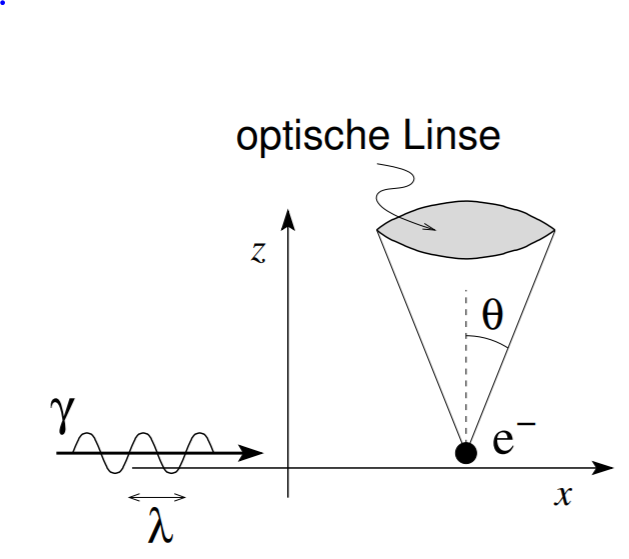
\includegraphics[scale=0.8]{8.PNG}
    \end{minipage}
    \begin{minipage}{0.5\textwidth}
        \captionsetup{font={Large}}
        \caption{X-ray microscope for observation of an electron (thought experiment).}
    \end{minipage}
    \label{fig:8}
\end{figure}
we build the Schrodinger wave mechanics from similar thought experiments
on (see, e.g., Feymann \& Hibbs).